\documentclass[tikz, crop, border=5pt]{standalone}
\usetikzlibrary{positioning,backgrounds,fit}
\usepackage{forest}

\usepackage{fontspec}
\usepackage{xeCJK}

\setmainfont{NotoSans}[
    Extension      = .ttf,
    UprightFont    = *-Regular,
    BoldFont       = *-Bold,
    ItalicFont     = *-Italic,
    BoldItalicFont = *-BoldItalic
]

\usepackage{color}
\definecolor{indianred1}{RGB}{255, 106, 106}
\definecolor{deepskyblue}{RGB}{0, 191, 255}
\definecolor{palegreen}{RGB}{152, 251, 152}
\definecolor{burlywood}{RGB}{222, 184, 135}
\definecolor{grey}{RGB}{129,130,132}

\begin{document}
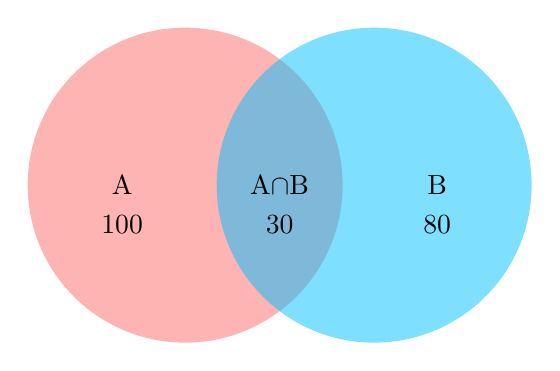
\begin{tikzpicture}
%VENN_BEGIN%
    % Basic parameters for circles
    \def\radius{2cm}
    \def\overlap{1.2cm}

    % Draw two circles
    \begin{scope}[opacity=0.5]
        \fill[indianred1] (-\overlap,0) circle (\radius);
        \fill[deepskyblue] (\overlap,0) circle (\radius);
    \end{scope}

    % Add labels
    \node at (-2,0) {A};
    \node at (2,0) {B};
    \node at (0,0) {A$\cap$B};

    % Add numbers
    \node at (-2,-0.5) {100};
    \node at (2,-0.5) {80};
    \node at (0,-0.5) {30};
%VENN_END%
\end{tikzpicture}
\end{document}
